Das Rastertunnelmikroskop (engl. Scanning Tunneling Microscope, kurz: STM) ist eine Methode der
Rastersondenmikroskopie, bei der eine dreidimensionale Aufnahme atomarer Oberflächen elektrisch
leitender Festkörper erstellt werden kann. Die Funktionsweise beruht auf dem quantenmechanischen
Tunneleffekt (siehe Abb. \ref{tunnel}): Wird eine sehr feine, leitende Spitze - idealerweise nur ein
Atom - bis auf wenige {\AA} an die Oberfläche heran gebracht und eine Spannung angelegt, fließt zwischen Spitze und
Oberfläche ein Strom. Durch die kurze Distanz ist die Tunnelbarriere, die das Vakuum darstellt,
endlich, und je nach Polung der Spannung können die Elektronen von der Spitze zur Oberfläche tunneln bzw.
umgekehrt. Der Strom ist dabei abhängig von der elektronischen Zustandsdichte der Spitze und der
Probe an dieser Stelle, von der angelegten Spannung sowie vom Abstand. Wird die Spitze über die
Oberfläche bewegt und Strom bzw.
Abstand gemessen, kann auf diese Weise ein topographisches Bild der Oberfläche mit atomarer
Auflösung erreicht werden. 

\begin{figure}[H]
\centering
\includegraphics[width=5cm]{TunnelEffekt.png}
\caption{\textit{Veranschaulichung des Tunneleffekts. Ein Elektron mit Energie $E_{e^-}$ kann nach
klassischen Gesetzen die Potentialbarriere $V$ mit $V>E_{e^-}$ nicht überwinden, tatsächlich besteht
jedoch nach quantenmechanischer Rechnung eine endliche Wahrscheinlichkeit dafür, das Teilchen
außerhalb der Barriere zu finden. Das Elektron durchtunnelt diese, wobei die
Aufenthaltswahrscheinlichkeit $|\Psi|^2$ innerhalb der Barriere exponentiell abklingt. }}
\label{tunnel}
\end{figure}

Eine der größten Hindernisse bei der quantitativen Beschreibung der Rastertunnelmikroskopie ist die
im Allgmeinen unbekannte Struktur der Spitze, sodass eine Beschreibung immer Annahmen und Näherungen
beinhaltet. Einer dieser Näherungen ist die von Tersoff und Hamann \cite{Ter83}, \cite{Ter85}, die
zu einer direkten Interpretation der STM Bilder als konstante lokale Oberflächenzustandsdichte führt.\\
Der Strom ist nach Störungstheorie erster Ordnung nach Bardeen \cite{Bar} gegeben durch

\[I=\frac{2\pi e}{\hbar}\sum_{S,P}
f(E_{S})[1-f(E_{P}+eU)]\cdot|M_{SP}|^2\delta(E_{S}-E_{P})\]

mit der Fermifunktion $f(E)$, der angelegten Spannung $U$, der Energie
$E_{S}$ des Zustandes $\psi_{S}$ ohne Tunneln sowie dem Tunnelmatrixelement $|M_{SP}|$
zwischen den Zuständen $\psi_{\mu}$ der Spitze und $\psi_{\nu}$ der Oberfläche

\[M_{SP}=-\frac{\hbar^2}{2m}\int d\vec{S}\cdot(\psi_{S}^*\nabla\psi_{P} -
\psi_{P}\nabla\psi_{S}^*) \]

wobei die Fläche $d\vec{S}$ dabei vollständig innerhalb der Vakuumbarriere liegen muss, die
Spitze und Probe trennt. Mit der Näherung kleiner Temperaturen und kleiner Spannungen $U$ ergibt
sich

\[I=\frac{2\pi e^2}{\hbar}U\sum_{S,P}|M_{SP}|^2\delta(E_{P}-E_{F}) \delta(E_{S}-E_{F})\]

mit der Fermienergie $E_F$. Da die Wellenfunktion $\psi_{\mu}$ der Spitze unbekannt ist, wird sie
nun folgendermaßen modelliert: Der Teil der Spitze, der der Oberfläche am nächsten ist, wird als
sphärischer Potentialtopf angesetzt (siehe Abb. \ref{spitze}). Dabei ist $R$ der Radius der Kugel
und $d$ ist der kürzeste Abstand zur Oberfläche. Das Matrixelement $|M_{SP}|$ wird
also lediglich für ein s-Orbital der Spitze ausgewertet, die d- und p-Wellenfunktionen werden
vernachlässigt. Weiterhin wird vereinfachend angenommen, dass die Austrittsarbeit von Spitze und
Probe gleich ist.

\begin{figure}[H]
\captionsetup{format=plain}
\centering
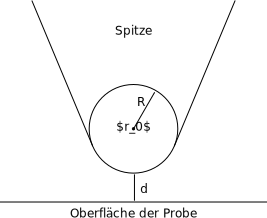
\includegraphics[width=5cm]{spitze.svg}
\caption{\textit{Schema des Tunnelkontakts nach Tersoff und Hamann. Die Spitze wird als sphärisches
Potential mit Radius $R$ und Abstand $d$ zur Probenoberfläche modelliert.}}
\label{spitze}
\end{figure}
 
 Die explizite Rechnung soll hier nicht ausgeführt werden (für Details, siehe \cite{Ter83}).
 Letztendlich erhält man für den Tunnelstrom $I$
 
 \[I=32\pi^3\hbar^{-1}e^2U\phi^2\rho_{S}(E_F)R^2\kappa^{-4}e^{2\kappa
 R}\cdot\rho_P(\vec{r}_0, E)\]
 
 mit der Zustandsdichte $\rho_{S}$ pro Volumen der Spitze, der Austrittsarbeit $\phi$, der inversen
 Abklinglänge $\kappa=\hbar^{-1}(2m\phi)^{1/2}$ sowie der Zustandsdichte der Probe
 $\rho_P(\vec{r}_0, E)$
 
 \[\rho_P(\vec{r}_0, E)=\sum_{P}|\psi_{P}(\vec{r}_0)|^2\delta(E_{P}-E_F).\]
 
 Wie erwartet gilt also
 
 \[I\propto U \rho_{s}(E_F) \rho_P(\vec{r}_0, E).\]
 
 Der Zusammenhang zum Abstand zwischen Probe und Spitze ergibt sich aus der
 Wellenfunktion der Probe, die im Vakuum exponentiell abfällt:
 
 \[|\psi_P(\vec{r}_0)|^2\propto e^{-2\kappa(d+R)}~~~\Rightarrow~~~I\propto e^{-2\kappa d}\]
 
% ok was weiß ich?
% - das mit der auflösung passt noch nicht so ganz, aber das kommt daher, weil die nur s orbitale
% betrachtet haben, was besser wird wenn man d und p orbitale mit dazunimmt, und außerdem das
% effektive potential, was binnig vorgeschlagen hat
